\subsection{Our computers}


\subsubsection{Rostand}
Rostand is a cluster of 640 nodes owned by Total S.A. company.
%
Each node is composed of 2 NUMA nodes with a Intel Xeon X5660 processor and 24~GB of memory per NUMA node (Fig.~\ref{fig:rostand}).
%
Each processor has 6 cores, for a total of 12 cores per node and 7680 cores for the entire cluster.

%   (-_-)   %
\begin{figure}[!ht]
        \centering
        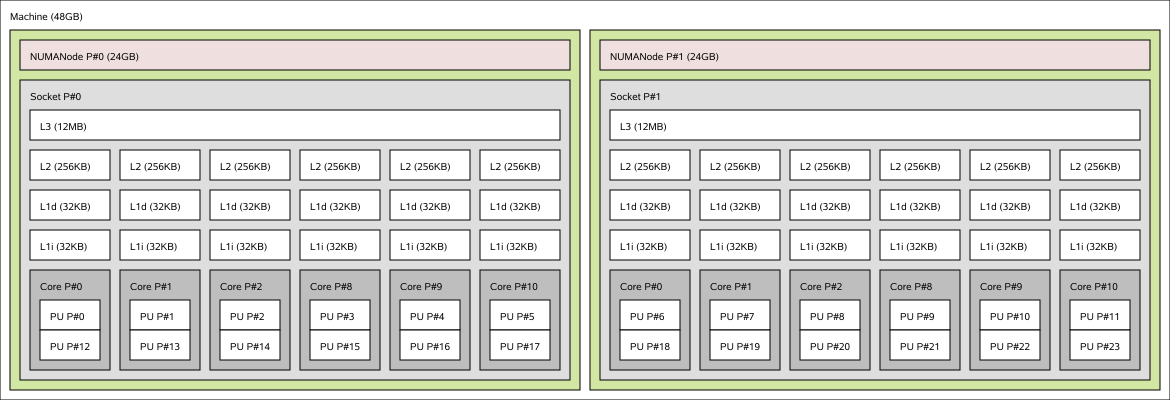
\includegraphics[width=\textwidth]{rostand_lstopo}
        \caption{Topology of one node of Rostand obtains with hwloc}
        \label{fig:rostand}
\end{figure}

\subsubsection{Manumanu}
Manumanu is an Altix UV100, this computer is composed of 20 NUMA nodes.
%
Each NUMA node is composed of Intel Xeon E7-8837 processor.
%
Each processor has 8 cores, for a total of 160 cores.
%
This computer is pretty interesting to test NUMA effects.
